
%(BEGIN_QUESTION)
% Copyright 2006, Tony R. Kuphaldt, released under the Creative Commons Attribution License (v 1.0)
% This means you may do almost anything with this work of mine, so long as you give me proper credit

A human operator is charged with controlling the temperature of water in a gas-fired water heater.  The ``setpoint'' (SP) is an ideal water temperature value held in the operator's mind, and the ``process variable'' (PV) of course is whatever the temperature gauge indicates:

$$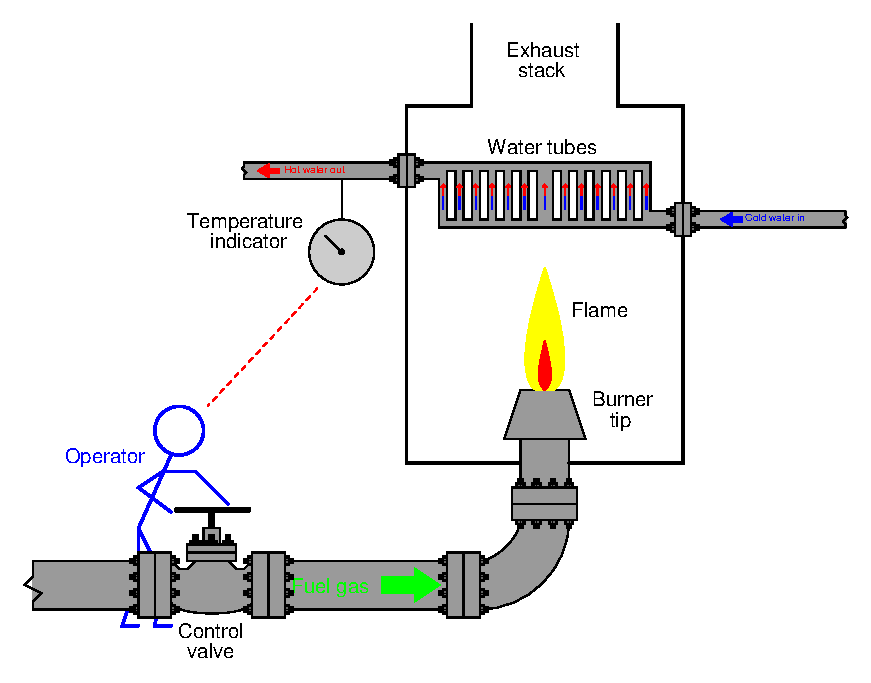
\includegraphics[width=15.5cm]{i01587x01.eps}$$

Imagine a situation where the water temperature is exactly at setpoint.  The operator is standing next to the gas control valve, bored, because there is nothing to do.  Then suddenly there is a demand for more hot water.  As the water flow through the heater increases, the outlet temperature begins to fall.  Noticing this decrease in PV, the operator opens the fuel valve by a proportional amount.  This causes the temperature to slowly climb back up to setpoint.  At some point in time, though, the water temperature settles at an equilibrium value that is less than setpoint.  The operator recognizes this and begins to become impatient, opening the valve a little bit more with each minute of time that goes by.  Eventually, after several additional ``opening'' motions of the valve, the water temperature rises to the setpoint value and stabilizes there.  Happy with the new situation, the operator resumes his previous condition of boredom.

\vskip 10pt

Now let us examine the operator's action in terms of how an automatic controller would handle the situation.  The operator's initial response to open the valve proportional to the amount of temperature decrease can be easily accounted for by {\it proportional} control action -- the name reveals it all.  But the operator's actions after noticing the PV settling at a temperature less than setpoint -- when he begins to feel impatient and opens the valve a little more each minute -- is definitely not characteristic of proportional control.  In fact, this action goes {\it against} what proportional control would do, by continuing to {\it increase} the valve's opening little by little even as temperature continues to {\it rise} to setpoint.

What the operator did was to examine how much error there was left between SP and PV, and also how long this condition of error persisted, and move the control valve accordingly.  Explain how the operator's action in doing this could be described as {\it integration} in the calculus sense of the word.

\underbar{file i01587}
%(END_QUESTION)





%(BEGIN_ANSWER)

I will let you discuss this with your classmates to arrive at an explanation!

%(END_ANSWER)





%(BEGIN_NOTES)

The operator {\it integrated} the error with respect to time to adjust the valve further and further open until there was no error left to integrate:

$$m = \int e \> dt + m_0$$

%INDEX% Control, integral: human operator perspective

%(END_NOTES)


